\documentclass{article}
\usepackage[utf8]{inputenc}
\usepackage[a4paper, headheight=14pt, left=1.75cm, right=1.75cm, top=1.25cm, bottom=1cm]{geometry}
\usepackage{amsthm, amsmath, mathtools, amssymb, physics, thmtools, thm-restate} % for math and physics commands and symbols.
\usepackage{parskip} % exchanges indentation for spacing between paragraphs.
\usepackage[catalan,english]{babel} % for Catalan language support.
\usepackage{color} % for colored text.
\usepackage{hyperref} % for hyperlinks.
\usepackage{xcolor} % for colored text.
\usepackage{caption} % for captions.
\usepackage{wrapfig}
\captionsetup[figure]{font=footnotesize,labelfont={footnotesize,bf}}

%% for references (hyperref)
\hypersetup{
  colorlinks = true,
  linkcolor = red!60!black, % color of internal links (sections, pages, etc.) 
  filecolor = cyan, % color for URLs which open local files
  % citecolor = green!70!black, %	color for bibliographical citations in text.     
  citecolor = green!40!black, %	color for bibliographical citations in text.     
  urlcolor = cyan, % color of URL links (mail, web) 
}
%%%%%%%%%%%%%%%%%%%%

\usepackage{bibliography} % for bibliography.

\pagestyle{empty} % Removes page numbers

% changes section style to subsection style
\makeatletter
\renewcommand\section{\@startsection{section}{1}{\z@}%
  {-3.5ex \@plus -1ex \@minus -.2ex}%
  {2.3ex \@plus.2ex}%
  {\large\bfseries}}
\makeatother

\renewcommand{\normalsize}{\fontsize{9.8pt}{12pt}\selectfont}

% change font size of subsections

% \hyphenpenalty=10000
% \exhyphenpenalty=10000

\begin{document}
% set language catalan
\selectlanguage{catalan}
\begin{center}
  \Large \textbf{Propagació numèrica dels errors dels\\satè\lgem its en òrbita terrestre}
\end{center}
\vspace{0.2cm}
% add author and supervisor in the same line but symmetric with respect to the center of the page
\begin{minipage}[t]{0.49\textwidth}
  \begin{flushleft} \large
    \emph{Autor:}\\[0.1cm]
    Víctor Ballester
  \end{flushleft}
\end{minipage}\hfill
\begin{minipage}[t]{0.49\textwidth}
  \begin{flushright} \large
    \emph{Supervisor:} \\[0.1cm]
    Josep Maria Mondelo
  \end{flushright}
\end{minipage}\\[0.2cm]


Des de l'inici de l'exploració de l'espai fins ara, l'entorn orbital de la Terra ha experimentat un augment significatiu de satè\lgem its, brossa espacial i altres elements relacionats amb l'exploració espacial. Aquesta contaminació a l'espai és motiu d'una preocupació creixent de la comunitat científica. A mitjans de l'any 2023 hi havia aproximadament 27.500 artefactes en òrbita terrestre \cite{web:spacetrack_cat}. D'aquests, uns 11.000 eren satè\lgem its actius; 2.300 eren peces de coets (és a dir, unitats de propulsió utilitzades per posar els satè\lgem its en òrbita); 13.700 eren satè\lgem its inactius (brossa espacial), i la resta eren objectes no classificats. Amb el pas dels anys, la probabilitat de co\lgem isió entre dues naus espacials augmenta de manera contínua. Ja s'han produït co\lgem isions greus en el passat, com ara el xoc a alta velocitat entre els satè\lgem its Iridium 33 i Kosmos-2251 el 2009 \cite{wiki:collision_cat}.

La dinàmica orbital al voltant de la Terra és molt complexa. L'aproximació kepleriana proporciona resultats precisos només durant poques hores. És per això que cal afegir millores en aquest model. Les pertorbacions importants de l'aproximació kepleriana són: el camp gravitatori real de la Terra (que no és keplerià perquè la Terra no és ni una massa puntual ni una esfera amb densitat constant); la resistència atmosfèrica; els efectes de tercers cossos (principalment el Sol i la Lluna), i la pressió de radiació solar. Els models més precisos (vegeu \cite{sgp4OrbitDet_cat}) inclouen totes aquestes pertorbacions i, fins i tot, algunes més, i són capaços de fer prediccions raonablement precises per a uns quants dies. Això fa possible mantenir un catàleg de naus espacials (tant actives com inactives) detectades a través d'una xarxa global heterogènia d'estacions d'observació, que poden ser òptiques (telescopis) o basades en radar \cite{web:spacetrack_cat,web:celestrak_cat}. Mantenir aquest catàleg actualitzat requereix observacions constants.

L'objectiu d'aquest treball és proporcionar una visió quantitativa de l'efecte que aquestes pertorbacions tenen de manera individual. Per això, s'han desenvolupat matemàticament els models necessaris \cite{montenbruck,vallado}. Primer de tot, s'ha pres com a referència un sistema on les lleis de Newton són vàlides. Ara bé, com que s'ha utilitzat un model de la Terra amb densitat no constant, en cada pas de la integració numèrica ha calgut situar els satè\lgem its als seus llocs exactes un cop projectats sobre la superfície terrestre. Com a conseqüència, s'ha hagut de considerar un altre sistema de referència no inercial lligat a la rotació de la Terra. Per tal de convertir les posicions dels satè\lgem its d'un dels sistemes a l'altre, ha calgut tenir present tots els moviments que experimenta l'eix de rotació terrestre: la precessió, la nutació i el moviment polar.

\begin{wrapfigure}[18]{r}{0.415\textwidth}
  \vspace{-0.35cm}
  \centering
  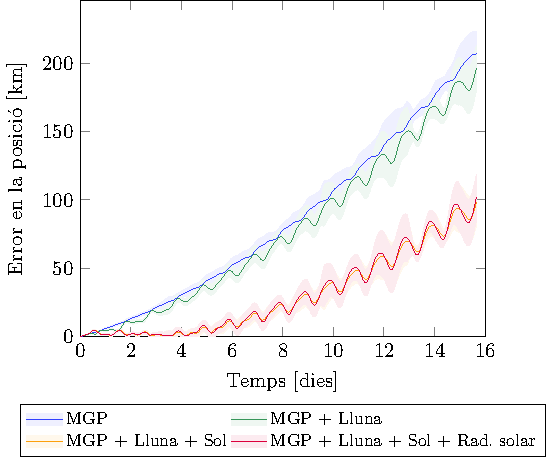
\includegraphics[width=0.415\textwidth]{Images/simulation/TDRS-3-cat.pdf}
  \caption{Propagació del satè\lgem it TDRS-3 usant el model geopotencial i  considerant les pertorbacions de la Lluna, el Sol i la pressió de radiació solar.}
  %\caption{Propagation of the TDRS-3 satellite considering the perturbations from the Moon, the Sun and the solar radiation pressure.}
  \label{fig:TDRS}
\end{wrapfigure}
Durant la simulació, no només s'ha considerat la força de la gravetat com a condicionant a l'acceleració del satè\lgem it, sinó que també s'han tingut present les quatre petites pertorbacions mencionades anteriorment. Cal esmentar que no s'ha afegit la interacció gravitatòria d'altres planetes, com ara Venus, Mart o Júpiter, amb els satè\lgem its en les nostres simulacions. Això és perquè, per als nostres propòsits, la seva influència és menyspreable en comparació amb l'ordre de magnitud de les pertorbacions del Sol i la Lluna.

Després de considerar exhaustivament tots els fenòmens significatius, s'ha dissenyat un model que els inclou i s'ha procedit a realitzar la simulació. Per integrar el sistema d'equacions diferencials s'ha utilitzat el mètode de Runge-Kutta 7(8), amb una tolerància relativa de $10^{-12}$. A més, s'han escollit tres zones orbitals molt diferents entre si per ser estudiades: els satè\lgem its d'òrbita baixa (LEO), que orbiten a altituds menors a 1.000 km; els satè\lgem its d'òrbita mitjana (MEO), que orbiten a altituds situades entre 1.000 i 35.780 km, i els satè\lgem its d'òrbita geoestacionària, que orbiten a distàncies al voltant dels 35.780 km per sobre del nivell del mar.

\vspace{-0.2cm}
\printbibliography[title={Referències}]
\end{document}